\chapter{Una suave introducción a GObject}
\label{oop-gobject}

En el capítulo anterior hemos aprendido a escribir código semi-orientado a objetos en C. Así es como se escriben las clases en GLib core. GObject avanza varios pasos en la programación orientada a objetos, con herencia, interfaces, funciones virtuales, etc. GObject también simplifica el paradigma de programación dirigida por eventos, con señales y propiedades.

Se recomienda crear sus propias clases de GObject para escribir una aplicación GLib / GTK. Desafortunadamente, el código es un poco detallado, porque el lenguaje C no está orientado a objetos. El código repetitivo es necesario para algunas funciones, pero no tenga miedo, existen herramientas y scripts para generar el modelo repetitivo.

Sin embargo, este capítulo da un paso atrás del capítulo anterior, es solo una pequeña introducción a GObject; explicará las cosas esenciales para saber cómo \emph{usar} una clase GObject existente (como todos los widgets y clases GTK en GIO). No explicará cómo \emph{crear} sus propias clases de GObject, porque ya está bien cubierto en el manual de referencia de GObject, y el objetivo de este libro no es duplicar todo el contenido de los manuales de referencia, el objetivo es más para que sirva de guía de introducción.

Entonces, para obtener información más detallada sobre GObject y saber cómo crear subclases, la documentación de referencia de GObject contiene capítulos introductorios: ``\emph{Conceptos}'' y ``\emph{Tutorial}'', disponibles en:

\url{https://developer.gnome.org/gobject/stable/}

Para explicar ciertos conceptos, se toman algunos ejemplos de GTK o GIO. Al leer este capítulo, se le anima a abrir Devhelp en paralelo, para mirar la referencia de API y ver por sí mismo cómo se documenta una biblioteca basada en GObject. El objetivo es que seas autónomo y puedas aprender cualquier clase nueva de GObject, ya sea en GIO, GTK o cualquier otra biblioteca.

\section{Herencia}
\label{oop-gobject-inheritance}

Un concepto importante de OOP es la herencia. Una clase puede ser una subclase de una clase principal. La subclase hereda las características de la clase padre, extendiendo o anulando su comportamiento.

La biblioteca GObject proporciona la clase base \lstinline{GObject}. Cada clase en GIO y GTK hereda, directa o indirectamente, de la clase base \lstinline{GObject}. Al mirar una clase basada en GObject, la documentación (si está escrita con GTK-Doc) siempre contiene una \emph{Jerarquía de objetos}. Por ejemplo, \lstinline{GtkApplication} tiene la siguiente jerarquía de objetos:

\begin{verbatim}
GObject
└── GApplication
    └── GtkApplication
\end{verbatim}

Significa que cuando crea un objeto \lstinline{GtkApplication}, también tiene acceso a las funciones, señales y propiedades de \lstinline{GApplication} (implementado en GIO) y \lstinline{GObject}. Por supuesto, las funciones \lstinline{g_application_*} toman como primer argumento una variable de tipo ``\lstinline{GApplication *}'', no ``\lstinline{GtkApplication *}''. Para convertir la variable en el tipo correcto, la forma recomendada es usar la macro \lstinline{G_APPLICATION()}. Por ejemplo:

\begin{lstlisting}
GtkApplication *app;

g_application_mark_busy (G_APPLICATION (app));
\end{lstlisting}

\section{Macros de GObject}

Cada clase de GObject proporciona un conjunto de macros estándar. La macro \lstinline{G_APPLICATION()} como se demostró en la sección anterior es una de las macros estándar proporcionadas por la clase \lstinline{GApplication}.

No todas las macros estándar de GObject se explicarán aquí, solo las macros útiles para \emph{usar} un GObject de una manera básica. Las otras macros son más avanzadas y generalmente son útiles solo cuando se subclasifica una clase GObject, cuando se crea una propiedad o una señal, o cuando se reemplaza una función virtual.

Cada clase GObject define una macro de la forma \lstinline{NAMESPACE_CLASSNAME(object)}, que convierte la variable al tipo ``\lstinline{NamespaceClassname *}'' y comprueba en tiempo de ejecución si la variable contiene correctamente un \lstinline{NamespaceClassname} objeto o una subclase del mismo. Si la variable es \lstinline{NULL} o contiene un objeto incompatible, la macro imprime un mensaje de advertencia crítico en la consola y devuelve NULL.

Un elenco estándar también funciona, pero la mayoría de las veces no se recomienda porque no hay comprobaciones de tiempo de ejecución:
\begin{lstlisting}
GtkApplication *app;

/* Not recommended */
g_application_mark_busy ((GApplication *) app);
\end{lstlisting}

Otra macro útil cuando se usa un GObject es \lstinline{NAMESPACE_IS_CLASSNAME(object)}, que devuelve \lstinline{TRUE} si la variable es un objeto \lstinline{NamespaceClassname} o una subclase del mismo.

% PARA HACER mostrar un ejemplo de una función que verifica sus argumentos con g_return?

\section{Interfaces}

Con GObject es posible crear interfaces. Una interfaz es solo una API, no contiene la implementación. Una clase GObject puede implementar una o varias interfaces. Si una clase GObject está documentada con GTK-Doc, la documentación contendrá una sección \emph{Interfaces implementadas}.

Por ejemplo, GTK contiene la interfaz \lstinline{GtkOrientable} que es implementada por muchos widgets y permite establecer la orientación: horizontal o vertical.

Las dos macros explicadas en la sección anterior también funcionan para interfaces. Un ejemplo con \lstinline{GtkGrid}:
\begin{lstlisting}
GtkWidget *vgrid;

vgrid = gtk_grid_new ();
gtk_orientable_set_orientation (GTK_ORIENTABLE (vgrid),
                                GTK_ORIENTATION_VERTICAL);
\end{lstlisting}

Entonces, cuando busca una determinada característica en la API para una cierta clase de GObject, la característica se puede ubicar en tres lugares diferentes:
\begin{itemize}
    \item En la propia clase GObject;
    \item En una de las clases padre en \emph{Jerarquía de objetos};
    \item O en una de las \emph{Interfaces implementadas}.
\end{itemize}

\section{Recuento de referencias}

La gestión de la memoria de las clases de GObject se basa en \emph{recuento de referencias}. Una clase GObject tiene un contador:
\begin{itemize}
    \item Cuando se crea el objeto, el contador es igual a uno;
    \item \lstinline{g_object_ref()} incrementa el contador;
    \item \lstinline{g_object_unref()} disminuye el contador;
    \item Si el contador llega a cero, el objeto se libera.
\end{itemize}

Permite almacenar el GObject en varios lugares sin necesidad de coordinar cuándo liberar el objeto.

\subsection{Evitar ciclos de referencia con referencias débiles}

Si el objeto A hace referencia al objeto B y el objeto B hace referencia al objeto A, hay un ciclo de referencia y los dos objetos nunca se liberarán. Para evitar ese problema, existe el concepto de referencias ``débiles''. Al llamar a \lstinline{g_object_ref()}, es una referencia ``sólida''. Entonces, en una dirección hay una referencia fuerte, y en la otra dirección debe haber una referencia débil (o ninguna referencia).

\begin{figure}
  \begin{center}
    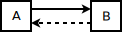
\includegraphics[scale=0.75]{imagenes/weak-ref.pdf}
    \caption{Using a weak reference to break the reference cycle between A and B.}
    \label{oop-gobject-weak-ref-schema}
  \end{center}
\end{figure}